\section{Results}
\label{sec:results}
The results follow the endpoints: first the accuracy curve with its onset and slope, then the classes on which the damage lands, the position of the native allocation, and finally probability quality before and after temperature scaling. The balanced arm reaches 39.57 percent balanced accuracy (36.70 to 42.53). Ten real patients with sixteen patches each reached 38.49 percent in \citet{queisler2026bracsMechanism}; twice the patch depth of this design adds about one point to the balanced reference, a plausible size for a cross-study comparison with different draws.

\subsection{Accuracy curve}
\label{sec:curve-results}
Balanced accuracy falls monotonically with the imbalance ratio, and it falls from the first step on (Table~\ref{tab:curve}, Figure~\ref{fig:curve}). At $\rho=2$ the damage is 1.15 points (0.14 to 2.35), so the onset of the grid is its smallest ratio, although the lower bound of the interval lies well below one point. The damage reaches 2.97 points (1.62 to 4.46) at $\rho=5$, 3.86 points (2.33 to 5.44) at $\rho=10$, and 7.98 points (6.01 to 10.17) at $\rho=100$, where the classifier has lost a fifth of its balanced accuracy. From $\rho=5$ on, every interval lies above the threshold. The three splits agree in direction and size: the damage at $\rho=100$ is 6.98, 8.67, and 8.28 points.

\begin{table}[htbp]
\centering
\small
\setlength{\tabcolsep}{4pt}
\renewcommand{\arraystretch}{1.15}
\begin{tabular}{@{}lrrrrrrr@{}}
\toprule
 & & & \multicolumn{2}{c}{Macro NLL (nats)} & \multicolumn{2}{c}{ECE (points)} & \\
\cmidrule(lr){4-5}\cmidrule(lr){6-7}
Arm & BA (\%) & Damage $\Delta$ & raw & scaled & raw & scaled & Temperature \\
\midrule
r1 & 39.57 & --- & 1.565 & 1.576 & 12.29 & 6.60 & 0.65 \\
r2 & 38.42 & \textbf{1.15} [0.14, 2.35] & 1.581 & 1.599 & 8.31 & 6.59 & 0.86 \\
r5 & 36.60 & \textbf{2.97} [1.62, 4.46] & 1.878 & 1.642 & 10.94 & 6.35 & 1.54 \\
r10 & 35.71 & \textbf{3.86} [2.33, 5.44] & 1.938 & 1.668 & 13.15 & 6.41 & 1.67 \\
r20 & 34.49 & \textbf{5.08} [3.34, 6.94] & 2.509 & 1.700 & 19.55 & 6.87 & 2.45 \\
r50 & 32.97 & \textbf{6.60} [4.76, 8.65] & 3.218 & 1.752 & 25.11 & 8.00 & 3.54 \\
r100 & 31.59 & \textbf{7.98} [6.01, 10.17] & 4.004 & 1.796 & 30.09 & 8.77 & 4.43 \\
\addlinespace
N ($\rho=6.7$) & 35.55 & \textbf{4.02} [2.68, 5.52] & 1.984 & 1.692 & 8.82 & 5.38 & 1.53 \\
\bottomrule
\end{tabular}
\caption{On BRACS, accuracy degrades from the mildest imbalance on, raw probability quality collapses, and temperature scaling removes almost all of the probability-quality loss. Balanced accuracy (BA) is test patient-macro balanced accuracy; the damage is $\mathrm{BA}(1)-\mathrm{BA}(\rho)$ in percentage points with paired 95\% bootstrap intervals, in bold where it meets the one-point criterion. NLL and ECE are shown without (raw) and with (scaled) the validation temperature; the temperature column is the mean fitted temperature over 30 fits, where values above one soften overconfident predictions and values below one sharpen underconfident ones. The 95\% intervals of the absolute BA levels are 5 to 6 points wide and are shared by all arms.}
\label{tab:curve}
\end{table}

\noindent The loss per doubling of $\rho$ is 1.18 points (0.90 to 1.50) over the whole grid, three times the 0.39 points of TCGA-UT \citep{queisler2026prevalenceTcga}. Unlike on TCGA-UT, the curve is close to linear in $\log\rho$: up to $\rho=10$ it loses 1.19 points per doubling (0.74 to 1.65), from $\rho=10$ to $\rho=100$ it loses 1.23 points (0.89 to 1.64), and the two intervals overlap widely. About half of the damage at $\rho=100$ is already present at $\rho=10$.

\begin{figure}[htbp]
\centering
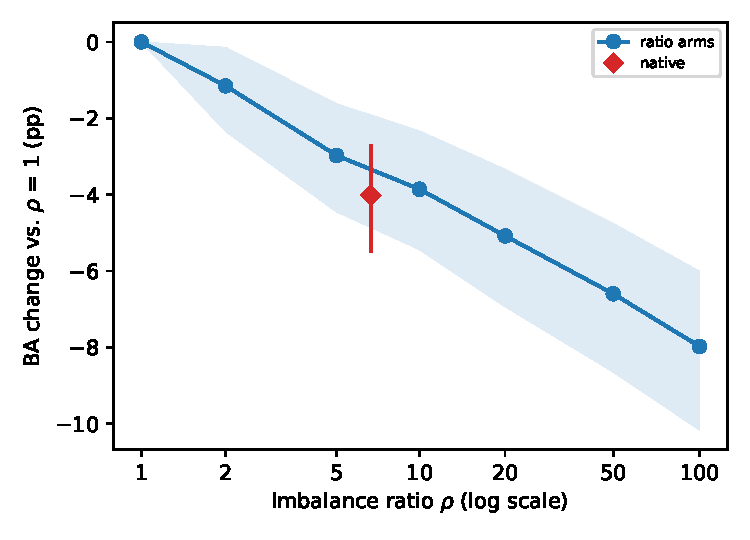
\includegraphics[width=0.6\textwidth]{discrimination_curve.pdf}
\caption{Balanced accuracy on BRACS degrades steadily, by about one point per doubling of the imbalance ratio. The line shows the change in patient-macro balanced accuracy relative to the balanced arm, with the ratio arms at their realized ratio and a shaded paired 95\% bootstrap band; the red diamond marks the native allocation at its realized ratio of 6.7.}
\label{fig:curve}
\end{figure}

\subsection{Where the damage lands}
\label{sec:rank-results}
The aggregate damage again results from recall moving from the rare to the frequent classes, but the transfer is far larger than on TCGA-UT (Table~\ref{tab:thirds}). In the balanced arm, the three head classes, two body classes, and two tail classes of the random rank order reach between 37 and 44 percent recall; with only seven classes and 30 draws, the rank groups do not average out class difficulty as completely as on TCGA-UT. With growing $\rho$, the head classes gain up to 15.0 points, whereas the body classes lose 17.7 points and the tail classes 32.7 points. At $\rho=100$ the tail classes reach 6.0 percent recall, so the classifier almost never predicts them. The body classes lose as well because, with seven classes, the exponential profile gives them only 120 and 56 of the 320 patches of the balanced share at $\rho=100$. Much of the redistribution happens early: at $\rho=2$ the tail classes already lose 12.7 points and the head classes gain 8.5.

\begin{table}[htbp]
\centering
\small
\renewcommand{\arraystretch}{1.15}
\begin{tabular}{@{}lrrrrrrr@{}}
\toprule
Rank group & r1 & r2 & r5 & r10 & r20 & r50 & r100 \\
\midrule
Head (3 classes) & 37.41 & 45.89 & 48.07 & 50.01 & 50.36 & 51.70 & 52.36 \\
Body (2 classes) & 43.66 & 39.65 & 36.75 & 34.48 & 32.94 & 29.37 & 26.00 \\
Tail (2 classes) & 38.73 & 25.98 & 19.23 & 15.50 & 12.23 & 8.49 & 6.04 \\
\bottomrule
\end{tabular}
\caption{Imbalance moves recall from the rare to the frequent BRACS classes, and the tail classes are almost never predicted at $\rho=100$. Mean patient-macro recall in percent of the head, body, and tail classes of each draw, by their assigned rank, averaged over 30 fits. The native arm is omitted because its class order is not the random rank order that defines the groups.}
\label{tab:thirds}
\end{table}

\subsection{Native allocation}
\label{sec:native-results}
The native class distribution of BRACS costs 4.02 points against the balanced arm (2.68 to 5.52), four times the threshold, although its realized ratio of 6.7 is modest. It lies on the ratio curve: interpolated at its realized ratio, the curve predicts a damage of 3.27 points, and the native arm falls 0.75 points below it ($-1.99$ to 0.47), a difference whose interval contains zero. The native profile has two levels rather than an exponential decay, with three frequent classes (IC, PB, DCIS) and four rare ones (N, ADH, FEA, UDH), and it assigns the rare share to specific lesion types, among them the atypical lesions ADH and FEA. Within the precision of this study, the realized ratio alone nevertheless places it on the curve, and the study finds no evidence that the native order of the classes costs more than a random order.

\subsection{Probability quality}
\label{sec:calibration-results}
Raw probability quality degrades far more than accuracy, and a single temperature again removes almost all of the degradation (Table~\ref{tab:curve}, Figure~\ref{fig:calibration}). Macro NLL rises from 1.56 nats in the balanced arm to 4.00 nats at $\rho=100$, an increase of 2.44 nats (1.73 to 3.26). The raw ECE is not monotone in $\rho$. The balanced arm is underconfident, with a mean temperature of 0.65 and a raw ECE of 12.29 points; mild imbalance lowers the ECE at $\rho=2$ by 3.98 points (0.33 to 6.74). From $\rho=5$ on the mean temperature exceeds one, so overconfidence takes over; the ECE returns above the balanced level at $\rho=10$ and rises to 30.09 points at $\rho=100$, an increase of 17.81 points (8.91 to 26.79) over the balanced arm. After temperature scaling, the increase at $\rho=100$ shrinks to 0.22 nats of NLL (0.17 to 0.27) and 2.17 points of ECE ($-1.94$ to 5.92), whose interval contains zero. Scaling therefore removes 91 percent of the NLL increase and 88 percent of the ECE increase. The remaining scaled NLL increase is resolved from $\rho=2$ on and follows the accuracy loss. In the balanced arm, scaling raises the test NLL slightly, from 1.565 to 1.576 nats, because the temperature is fitted on a validation partition of only about 24 patients. The native arm follows the same pattern: its raw NLL exceeds that of the balanced arm by 0.42 nats (0.28 to 0.60) and its scaled NLL by 0.12 nats (0.08 to 0.16), while its ECE differs from the balanced arm by $-3.47$ points raw ($-9.55$ to 4.02) and $-1.22$ points scaled ($-4.59$ to 1.03).

\begin{figure}[htbp]
\centering
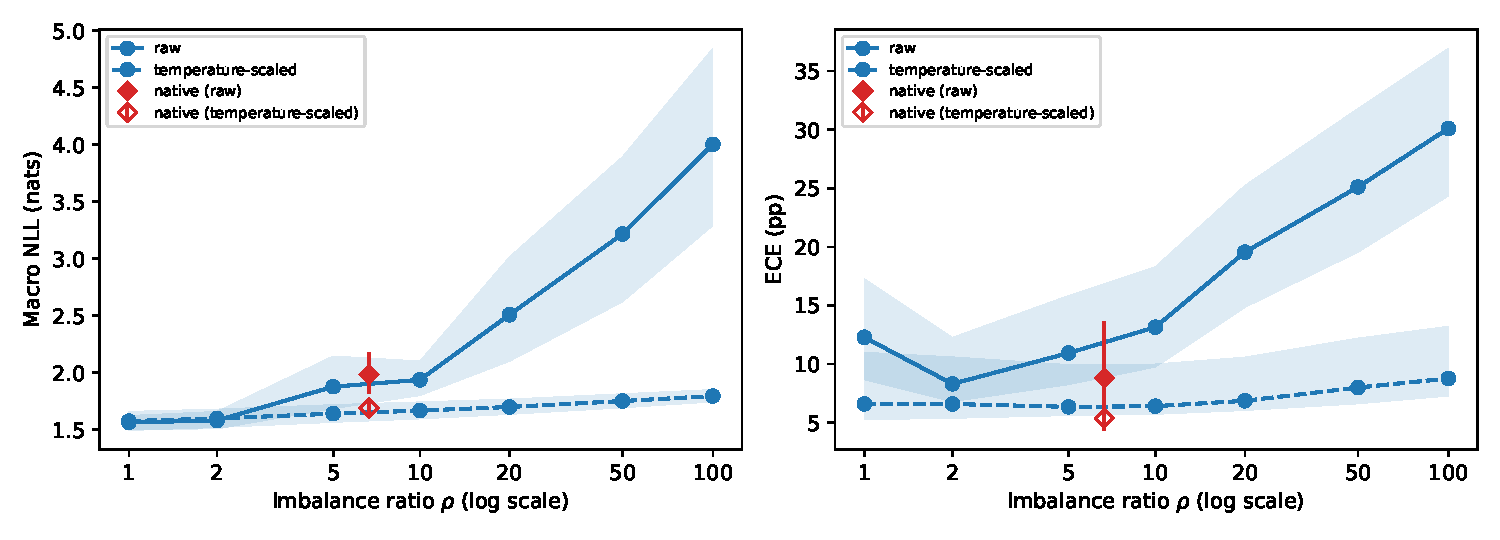
\includegraphics[width=\textwidth]{calibration_curve.pdf}
\caption{Raw probability quality on BRACS collapses with imbalance but recovers almost completely under temperature scaling. Left: macro NLL; right: ECE; both raw (solid, filled) and after validation temperature scaling (dashed, open). Blue lines connect the ratio arms at their realized ratio, with shaded paired 95\% bootstrap bands; the red diamonds mark the native allocation at its realized ratio of 6.7.}
\label{fig:calibration}
\end{figure}

The fitted temperatures and the selected regularization show the source of the overconfidence. The temperature rises from 0.65 in the balanced arm to 4.43 at $\rho=100$, so predictions must be softened by more than a factor of four. The balanced arm selects $\lambda=1$ or 10 in all 30 fits, whereas $\rho=100$ selects $\lambda\leq10^{-3}$ in 11 of 30 fits and the smallest grid value, $10^{-6}$, in 4. Refitting these four boundary fits with $\lambda$ down to $10^{-10}$ shows that the grid boundary constrains three of them: their validation balanced accuracy keeps rising below $10^{-6}$, by up to 0.38, 0.83, and 1.62 points, whereas the fourth is lower at every smaller value. Weak regularization lets the logits grow, which produces overconfident errors on the rarely predicted tail classes and explains the large raw NLL. As on TCGA-UT, the study does not separate this effect of model selection from the direct effect of the skewed class prior on confidence.

\section{Discussion}
\label{sec:discussion}
Of the three readings fixed in Section~\ref{sec:evaluation}, the results select the second, in a much stronger form than on TCGA-UT: prevalence alone damages discrimination on BRACS from $\rho=2$ on, by about one point per doubling, and by 7.98 points at $\rho=100$. The third reading is not supported, because the native allocation lies on the curve. The contrast with TCGA-UT is large. At $\rho=10$, the tail classes of both datasets keep about eight patches per patient, yet the damage is 4.02 points on BRACS against 0.57 on TCGA-UT \citep{queisler2026prevalenceTcga}; at $\rho=2$, where the tail keeps 22 patches per patient, BRACS already loses more than TCGA-UT does at $\rho=20$. The loss of per-patient support in the tail therefore cannot account for the BRACS damage by itself. A more likely source is the overlap of the BRACS classes. When classes overlap as much as a balanced accuracy of 40 percent implies, a skewed training prior shifts the decision boundaries between neighbouring lesion types far into the rare classes, whereas well-separated cancer types keep their boundaries almost regardless of the prior. The steeper profile of seven classes, with a factor of 2.15 between neighbouring ranks at $\rho=100$, adds to this. The study does not test the overlap explanation directly.

For the prevalence factor on BRACS, the curve refines the benchmark's three-allocation readout. The benchmark measured 4.30 to 13.23 points of concentrated severe-imbalance damage across tail assignments \citep{queisler2026benchmarkResults}; the 7.98 points at $\rho=100$, averaged over random class orders, lie inside that range. Because the benchmark also changed the patient pool, budget, and classifier, the magnitudes are not directly comparable, but both place severe prevalence damage on BRACS at several points. The native distribution costs 4.02 points, which is of the same size as the 4.80-point gain from five to twenty patients per class on BRACS \citep{queisler2026bracsMechanism}. On TCGA-UT, the native prevalence cost was about an eighth of the corresponding patient-count gain. On BRACS, class prevalence and patient count are therefore deficits of comparable size, and a long-tailed BRACS training set would need a prevalence correction even at adequate patient support.

Calibration behaves as on TCGA-UT, only more extremely. The raw NLL rises about 2.6-fold at $\rho=100$ and the ECE about 2.4-fold, while one validation temperature removes almost all of both increases. The calibration damage of imbalance on BRACS is thus again mostly a uniform overconfidence, amplified by weakly regularized models that validation accuracy selects under strong imbalance, and not a class-specific distortion. Prevalence-based corrections such as class weighting or threshold moving \citep{buda2018systematic} are more promising for discrimination on BRACS than on TCGA-UT, because much of the lost tail recall appears to be a boundary shift that a prior correction targets; for probability quality, they would again have to beat a temperature-scaled baseline.

With this study, the prevalence factor is measured on both datasets of the series. The remaining split studies vary patch count per class at fixed prevalence and patient count at fixed patch count, one factor at a time and with the same plain baseline, to show which of the benchmark's factors carries the damage it measured.

\section{Limitations}
\label{sec:limitations}
Each ratio moves the class prior and the tail support together, because the total budget is fixed; the study does not separate the effect of prevalence as such from the smaller per-patient patch count of the tail classes. The comparison with TCGA-UT at matched tail support argues that the prior carries most of the BRACS damage, but a design at fixed tail support would test this directly. The study uses ten patients per class instead of twenty, because only 10 to 13 ADH patients per training split reach 160 patches; the ADH patients therefore hardly change between draws, and the draws are less independent for this class than for the others. The curve describes imbalance at this fixed patient support and says nothing about the combination of rare classes with few patients.

The test and validation partitions hold only about 24 patients per split, which makes the ECE estimates wide and the temperature fits noisy; the non-monotone raw ECE at small ratios is resolved only at $\rho=2$. In three of the 30 fits at $\rho=100$, validation would have selected a weaker regularization than the grid allows; how this affects the reported damage and calibration is not measured. The rank groups contain two or three classes, so their recall mixes the imbalance effect with the difficulty of the particular classes that drew each rank. The native arm is a single allocation, and its agreement with the curve does not show that every class order behaves like a random one. All results are conditional on frozen Virchow2 features, multinomial logistic regression, BRACS, and three overlapping splits.
